\chapter{The ScienceIE Task: Design and Implementation}

To complete the ScienceIE task, the plan was made to have one Java project containing three sub systems, where each of which could be called independently. As such, this section shall step through each subtask's design and implementation in order, beginning with a description of the preprocessing that was implemented, as it is generic to all subtasks.

After this section has finished describing the design and implenetation of the varous algorithms used in this project, the following section shall describe the results associated with them.

\section{Data Preprocessing}
To support processing in later systems, all data (development, training and test) had to be preprocessed. The idea of this piece of computation is to prepare the data for analysis, and to also reduce computation time (doing this process once for the entire system rather than once for each sub system). To further reduce experiment run time, Java serialisation was also used to save all the following preprocessing information for later retrieval.

In Java, for each paper file from ScienceIE, a \texttt{Paper} object was constructed. This held many important pieces of information about the paper in question, including location on disk, text extracted from its source file, and all preprocessing information. \texttt{Paper} itself is a \textit{plain old Java object}, only holding information and is an abstract class, with \texttt{TextPaper} and \texttt{PDFPaper} classes extending from it which could be instantiated. These extended classes inherited the data storage features and utilities from \texttt{Paper}, but their constructors are customised to extract information from their given type of file:

\begin{itemize}
	\item \texttt{TextPaper} is for \texttt{.txt} files and simply extracts the text from the document. It sees the title of the text document as the title of the paper.
	\item \texttt{PDFPaper} is for \texttt{.pdf} files. This uses Apache PDFBox\footnote{\href{https://pdfbox.apache.org/}{https://pdfbox.apache.org/}} (imported through Maven\footnote{\href{https://pdfbox.apache.org/2.0/dependencies.html}{https://pdfbox.apache.org/2.0/dependencies.html}}) to extract the text from a PDF. The title, once again, is the title of the document. As alluded to earlier, with the ScienceIE test set not only being just text files but also being short documents, longer PDF papers was not usually used, so little development to properly sanitise PDFs happened, meaning all titles and references were also captured in this text extraction. If more PDF files were to be processed this would have been looked at, however, due to its lack of use the time needed to fix this was deemed not worth it.
	\item It was initially planned that there would be a \textit{HTML} and \textit{WebPDF} classes although, for similar reasons to why the \texttt{PDFPaper} text extraction was not developed further, these two classes were never implemented. The main reason for wanting them was to later support the POC system, as this would allow that system to dynamically grab papers from the web and add them to itself. Importing of papers to the POC system shall be discussed later at a more relevant time.
\end{itemize}

The bulk of the preprocessing came in the form of using a parser to calculate the parse tree of a text. As discussed, many teams at ScienceIE used spaCy. As the plan for this project was to complete it in Java (creating a single, self contained system) the Stanford CoreNLP package was used \cite{Manning2014} (imported through Maven\footnote{\href{https://stanfordnlp.github.io/CoreNLP/download.html}{https://stanfordnlp.github.io/CoreNLP/download.html}}). While offering a range of useful NLP features, the main ones utilised by the project were tokenization and finding the parse tree of the text (which naturally included POS tagging). An \texttt{Annotator} class was constructed which accepted a \texttt{Paper} input and annotated the text contained using the CoreNLP library.

Further processing on this information was also completed, where (at the time of saving the CoreNLP parse information) a token \textit{map} was created. This \textit{map}'s key set was all tokens present in the document, with the associated value being the number of times the token was in the document. This was to help when calculating TF-IDF scores later in processing.

The final part of preprocessing was to load existing annotation information. Of course this was only possible for ScienceIE data, which were all supplied with the relevant \texttt{.ann} files in BRAT format. These records were loading into a list of \texttt{Extraction} abstract entities, where each entry to the list could be either of a \textit{KeyPhrase} or \textit{Relationship} extending type, which each held all the information supplied in the annotation files (including classifications, the types of relations and more).

\section{Subtask A - Key Phrase Extraction}
Subtask A at ScienceIE was considered the hardest, reinforced by both the maximum and average scores for each independent subtask. This paper dedicated most of its NLP effort to this task out of the three subtasks as this is currently the hardest part of information extraction (out of the given subtasks) under current research. 

Two attempts at this subtask were made. Initially, a \textit{safer} design involved a SVM which considers some of the key features about key phrases suggested in the literature around this topic. Then, an even more experimental trail shall be described which involves clustering based around Word2Vec similarities between words in a document. 

\subsection{Method 1: Support Vector Machine}
Inspired by the highest success at ScienceIE, a SVM approach was adopted to attempt to provide a solution to subtask A. Initially, a small set of support vectors were selected and tested, with more being added as research continued.

\subsubsection*{Processing Data}
Two approaches were considered when designing the input and output data. One was based around passing each token in individually and in order, while the other was based around using the parse information obtained by using CoreNLP to pass sections of a sentence. 

Working with each individual token was selected for several reasons. Firstly, it was very easy to simply iterate through every token in a document in turn. Furthermore, the CoreNLP data is still available (evidences as that is what returns the tokens of the document) and can be passed to the SVM to be used when calculating support vectors. While using sections of a sentence should help keep any key phrase extracted more semantically correct (i.e. it should avoid missing the end of a noun phrase by accident which a check could be added for anyway), it poses a large issue: Any section selected as a key phrase would likely be \textit{locked down} as such to the specific tokens inside that section, meaning there may be no way to get rid of excess information or added extra if the gold standard key phrase requires something slightly different to the key phrase chosen by the SVM. In terms of extra information needed, a system could be implemented to join adjacent key phrases but that would like see extra information over what is needed being included. If, to try and solve this issue, some system which could extend or retract by a token or two was implemented, it is getting closer to the original option anyway where the system is processing the entire document as individual phrases. Therefore, a system based around processing each token individually was decided upon.

This resulted in a total of 65447 different training points (the total number of individual tokens in all of the training data).

\subsubsection*{Defining Features}
It is clear that current trends view the position of key phrases are very important in the document and should definitely be considered when trying to learn how to predict them. A tokens proximity to other tokens semantically and as part of the document as whole seem to significantly help us identify where key phrases lie. Furthermore, some attributes about individual phrases also seem to play a large part. For example, the length of the word is a valid feature to evaluate, as the average length of a key phrase token (7 characters) is slightly different to the average of all key phrases (8 characters). 

\begin{table}
	\centering
	\begin{tabular}{ C{7cm} | c }
		\textbf{Feature Description} & \textbf{Value Range} \\
		\hline
		The length of the token divided by the maximum token length in the training set. & \texttt{svLen} $\in$ $\mathbb{R}$,  0 $\leq$ \texttt{svLen} $\leq$ 1 \\
		\hline
     	Whether the token is a noun (using Part-Of-Speech tagging). & \texttt{svPos} $\in$ \{0, 1\} \\
     	\hline
     	The TF-IDF score of the token. & \texttt{svTfIdf} $\in$ $\mathbb{R}$,  0 $\leq$ \texttt{svTfIdf} $\leq$ 1 \\
     	\hline
     	The token index divided by the number of tokens. & \texttt{svDepth} $\in$ $\mathbb{R}$,  0 $\leq$ \texttt{svDepth} $\leq$ 1 \\
     	\hline
     	The token index in the current sentence divided by the number of tokens in the sentence. & \texttt{svDepthSentence} $\in$ $\mathbb{R}$,  0 $\leq$ \texttt{svDepthSentence} $\leq$ 1 \\
     	\hline
		Whether the token is in the first sentence of the paper. & \texttt{svFS} $\in$ \{0, 1\} \\
		\hline
     	Whether the token is in the last sentence of the paper. & \texttt{svLS} $\in$ \{0, 1\} \\
     	\hline
     	Whether the previous token was part of a key phrase. & \texttt{svLWKP} $\in$ \{0, 1\} \\
	\end{tabular}
	\caption[Initial Key Phrase SVM Features]{Initial key phrase support vector features used. A set of these features is generated for each token. When defining the value range, the variable is named as it is in the Java code.}
	\label{table:kpinitsvs}
\end{table}

Thankfully, the idea behind using an SVM is to find what separates key phrases from just normal phrases. Therefore, I was able to create an initial range of features, as defined in table \ref{table:kpinitsvs}. Here it is evident most of the features are based around trying to gather information as to the whereabouts of the token. It also, importantly, considers the sequence of key tokens.

\subsubsection*{Training}
To train the SVM, a \textit{problem} must be created. The \textit{problem} contains an array of vectors, where the vector is the set of features described above. Each of these data points must be labelled. The label is what we are trying to predict on the test data, so here the label is where or not the token is a key phrase (\texttt{0} for \textit{normal}, or \texttt{1} for key phrase). 

\subsubsection*{Model Selection}
As the nature of the data is unknown, an educated guess can be made as to which kernel to use. A common kernel to begin working with is the \textit{Radial Basis Function} (RBF) kernel \cite{Chih-WeiHsuChih-ChungChang2008}. This is because it can handle non-linear data, which it is assumed the training data here is to be. The RBF kernel function to find the similarity between two data points is listed below:

\begin{equation*}
K\textsubscript{RBF}(x_i, x_j) = exp(-\gamma||x_i - x_j||^2)
\end{equation*}

\noindent There are two parameters which can be configured and tuned to optimise performance of the SVM:
\begin{itemize}
	\item The cost \textit{C} parameter. This influences the misclassification allowance, where a small value lets the SVM select a large hyper-plane for separating data but allows for more misclassification, and a large value will allow the SVM to attempt to find a smaller hyper-plane that has less misclassification. Several values will be explored, of the set \{5, 50, 100, 200\}.
	\item The RBF kernel has a single parameter $\gamma$. From the same source that recommended the RBF kernel, as a initial value the SVM shall be configured to 0.5, as this is 1 divided by the number of features (we have 2 labels). However, other values shall be explored to attempt to find the best accuracy, and these values shall be \{0.25, 0.5, 1\}.
\end{itemize}

\subsubsection*{Development}
Having decided on how to use the concept of an SVM, there was a need for a concrete implementation. The idea of implementing an SVM was considered, however, with a responsibly high implementation complexity and a high risk of getting something subtly wrong (therefore being hard to detect and fix) a pre-existing solution was searched for. Furthermore, with the author having never handled an SVM before, a pre-existing solution with additional usage information was desired. This is why libsvm was chosen to be used in this project.

To allow for further SVM usage, an abstract \texttt{BaseSvm} was implemented so that any SVM created as part of this project can extend from this and use these functions generic to all SVMs. This has a default configuration set, a generic training method (calling \texttt{.svm\_train(problem, configuration)}), a generic predict method and a \texttt{.makeNewNode(index, value)} method. This \textit{makeNewNode} method creates a feature for a data point in the format the SVM library can understand (a \textit{vector} is an array of \texttt{svm\_node}s). It also validates the value of the feature, setting it to 0 is somehow an infinite or \textit{NaN} has been passed in. 

This base SVM class also holds a cross validation function (\texttt{.doCrossValidation(\textit{C}, $\gamma$)}), which runs the cross validation procedure and returns the accuracy as a percentage.

From the above, the \texttt{KeyPhraseSVM} class was created which contained the functionality to build the required feature vectors of input data and add labels to the training data, which completed the requirements of the SVM.

To actually produce key phrases for a \texttt{Paper} object, once a token was \textit{predicted} to be part of a key phrase, its start and end position was noted. The following sequence of tokens would all have their status of key phrase or not key phrase predicted, and while there is a string of tokens predicted to be key phrases, the end position is updated to cover this range of tokens in the original document. Once a token is predicted to not be a key phrase, the \texttt{.makeKeyPhrase} method of \texttt{Paper} is called with the start and end positions of the tokens to be inside the key phrase, which creates the \texttt{KeyPhrase} object.

\subsubsection*{Additional Features and Post Processing}
While working on development of the key phrase SVM, further features were considered and implemented. To evaluate how effective they were, a baseline score was achieved and then each of these were added idea by idea to test if they increased the system performance or not. The additional items, in order, are listed in table \ref{table:kpextsvs}. 

\begin{table}
	\centering
	\begin{tabular}{ C{7cm} | c }
		\textbf{Feature Description} & \textbf{Value Range} \\
		\hline
		The Word2Vec distance from the given token to "task". & \texttt{svTask} $\in$ $\mathbb{R}$,  0 $\leq$ \texttt{svTask} $\leq$ 1 \\
		\hline
		The Word2Vec distance from the given token to "process". & \texttt{svProcess} $\in$ $\mathbb{R}$,  0 $\leq$ \texttt{svProcess} $\leq$ 1 \\
		\hline
		The Word2Vec distance from the given token to "material". & \texttt{svMaterial} $\in$ $\mathbb{R}$,  0 $\leq$ \texttt{svMaterial} $\leq$ 1 \\
		\hline
		The depth of the token in the parse tree for its parent sentence, divided by the maximum depth of any token in that sentence. & \texttt{svParseTreeDepth} $\in$ $\mathbb{R}$,  0 $\leq$ \texttt{svParseTreeDepth} $\leq$ 1 \\
		\hline
		Whether or not the token is a stop word. & \texttt{svIgnoreWord} $\in$ \{0, 1\} \\
	\end{tabular}
	\caption[Additional Key Phrase SVM Features]{Additional features to be calculated for each token added to the SVM. These were implemented in order and their benefit or reduction in performance is measured.}
	\label{table:kpextsvs}
\end{table}

The initial three focus on Word2Vec's \texttt{.similarity(word1, word2)} method, which finds the distance between two words in the Word2Vec space. The distances chosen were to the three types of classification laid out in the task description. The theory behind this is: as we are looking for tasks, processes and materials, words which are closely related to these concepts may be likely to have a higher similarity to those words in Word2Vec's vector space. Including this information as a feature in the SVM may help distinguish those data points which should be selected as key phrases (as they may be particularly close to one of the three target concepts).

Next, the parse depth of the token is considered. The idea of this is that if you imagine a parse tree, the leaves that are further away from the original sentence (has more branches leading to them) may generally be the more important parts of the sentence, as the other parts of the sentence (leaves less far down the tree structure) simply lead up to the key phrase and add extra information. Therefore, this should test to see if how \textit{central} a token is contributes to whether it should be seen as a key phrase.

Finally, there is a flag to described whether the token is a stop word. This should work with the TF-IDF feature described earlier to help identify words that are unimportant and should not be included in key phrases.

Along side these features, the results produced as part of development and manual analysis of the key phrases created gave incentive to \textit{tidy up} the key phrases with some post processing. This was to try to remove unwanted parts of key phrases, or bad key phrases entirely, and in conjunction with the above features, the following post processes were applied:

\begin{itemize}
	\item \textit{TF-IDF filter} - In an attempt to remove key phrases which were effectively just \textit{noise}, each key phrase was treated as a candidate key phrase and would only become a true key phrase if the total TF-IDF of the tokens inside of it was above 0.02. This value was set by reviewing the key phrases produced in earlier runs, calculating their TF-IDF values, ordering them and finding the first key phrase that had suitable words (what we'd want to see in a key phrase) in it. Rounded slightly down, this value was set as a threshold and removed all extremely low TF-IDF key phrases.
	\item \textit{Sanitisation on creation} - When a new key phrase was found by the SVM, the \texttt{.makeKeyPhrase} method is called. This method was amended to try to only produce well formed key phrases. This includes attempting to remove redundant symbols, blank space and stop words at the start and the end of the key phrase. The goal was to try to close the gap between strict and inclusive evaluation by removing some of the redundant information. Empty key phrases were also discarded.
	\item \textit{Final sanitisation changes} - The sanitisation added to the \texttt{.makeKeyPhrase} was revisited. The previous changes were refined and improved, and it was ensured all key phrases have some content in them (including support for special scientific characters such as "$\alpha$"). A new process added here was the splitting of key phrases if there is a bracket half way through the phrase. This creates two, more semantically correct key phrases (as originally, either side of the bracket would have been from different parts of the sentence), where at least one is more likely to be correct as no gold standard key phrase go across a bracket boundary and doesn't return later. 
\end{itemize}

Through some analysis of the output, the final changes to sanitisation also gave this system the opportunity to match obvious synonyms: If the original key phrase was "Support Vector Machine (SVM", the two split phrases would be "Support Vector Machine" and "SVM". A simple check was implemented to see if the capitalised characters of the first phrase ("Support Vector Machine" would be filtered to "SVM") were part of the second and vice versa, and if so a synonym relation was drawn between the pair of key phrases. 

\subsubsection*{Cross Validation}

\begin{figure}
	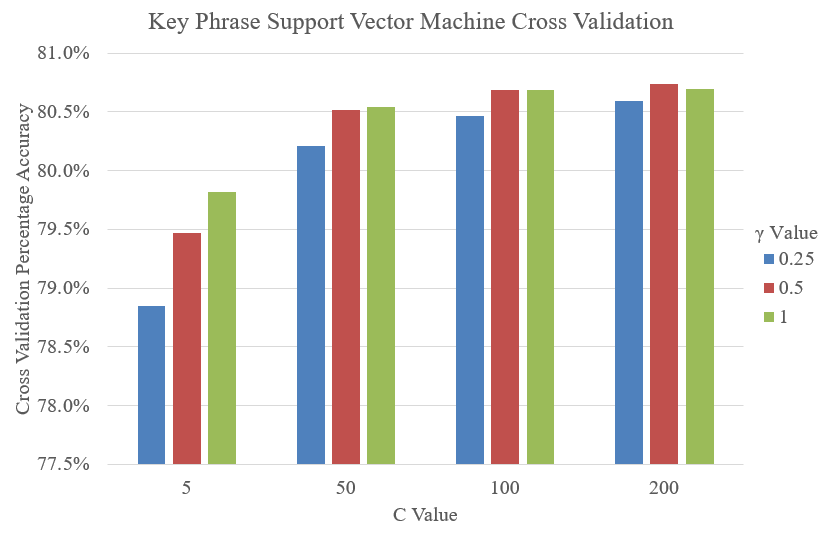
\includegraphics[width=\textwidth]{img/kpsvmcrossvalidation.png}
	\caption[Key Phrase SVM Cross Validation]{The cross validation results on the key phrase SVM. These were completed with all initial features and all extension features in place.}
	\label{figure:kpsvmcv}
\end{figure}

Cross validation is an important part when trying to optimise performance of an SVM. It allows for tuning key parameters by running repeated tests. Rather than using the testing data, which could introduce bias, the training data is split up into \textit{n} folds (or groups of data from within the training set). \textit{n = 5} folds were used in this instance. In turn, the SVM is trained with 4 of the 5 folds and then evaluated against the remaining fold. This is repeated for all combinations of folds and then the accuracy of the SVM can be calculated. A higher accuracy should mean better performance, although there is the problem of over fitting to consider. If the model is built to run perfectly on the training data, real world performance may actually suffer. This is why we cannot stop testing the SVM after just cross validation, as evaluating against the unseen test set will tell us how well it really performs. 

The values discussed for \textit{C} and $\gamma$ were used in cross validation and their outputs compared. The cross validation results can be seen in figure \ref{figure:kpsvmcv}. As show by this chart, very little change is accuracy is observed. There is a upward trend as \textit{C} and $\gamma$ increase, but this appears to plateau as higher values are evaluated. No smaller values need testing as (given the trend continues) the accuracy will significantly diminish. In terms of increasing the values, there is potential for extremely small gains; however, the return from increasing these values will be almost worthless and the training time required as the \textit{C} value increase significantly rises, as the SVM is working harder to find a better fitting hyperplane. Therefore, \text{C = 100} and \textit{$\gamma$ = 0.5} shall be used when completing full experiments. While, a \textit{C} value of 200 is 0.05\% more accurate with the same $\gamma$ value, the training time is roughly doubled (from some hours to many hours) and the reward is not deemed worth it.

\subsubsection*{Self Evaluation}
A problem referenced in the literature review was evaluation of key phrase extraction. What was discussed is how to classify good and bad systems. It is easy to accurately say how well a system performed compared to a set of gold standard data, but this paper considers whether that is enough to say whether a given extraction system is a success or not.

% TODO Maybe talk abbout existing solutions in cross bracket metrics

\begin{table}
	\centering
	\begin{tabular}{ C{3cm} | C{10cm} }
		\textbf{Strictness} & \textbf{Description} \\
		\hline
		Very strict (\texttt{REALLY\_STRICT}) & Both the predicted key phrase string and its boundaries need to match the gold standard string and boundaries. This is of equivalent strictness to the \textit{BRAT} evaluation completed by the ScienceIE scripts. \\
		\hline
		Matching (\texttt{STRICT}) & Just the predicted key phrase string needs to match the gold standard string. \\
		\hline
		Inclusive matching (\texttt{INCLUSIVE}) & The predicted key phrase string must be equal too or include the gold standard string. \\
		\hline
		Generous matching (\texttt{GENEROUS}) & The predicted key phrase string can include the gold standard string, or the gold stand string can include the predicted. \\
	\end{tabular}
	\caption[Strictness Descriptions for Self Evaluation of Key Phrases]{The strictness levels used in self evaluation of key phrase extraction. The \textit{strictness} title also includes the \texttt{Strictness} enumeration value as in the Java code for reference.}
	\label{table:strictness}
\end{table}

Therefore, in preparation for evaluation, several metrics will be used. The metric titles and descriptions can be seen in table \ref{table:strictness}. The point of these different metrics for deciding whether a prediction is good or not, is to try to capture a sense of how much of the information we are aiming to extract we actually achieve, potentially foregoing some extra information. Of course, a metric equal to that of the ScienceIE test scripts is included so we can get an expected value for when running with those scripts and a good comparison value for the other metrics used in this paper.

Firstly, the \textit{matching} variant is believed to be perfectly reasonable: it results in exactly the same textual information output, it is merely less concerned with the informations original location. A higher score in this should be considered very positive, as when a reader is looking through key phrases extracted from various papers (for example when trying to pick one out that is useful to them), they likely don't care exactly which sentence the text came from. Even when looking at an individual paper as part of the ScienceIE data set, origin sentence likely doesn't matter as the documents are short and it should be easy to see where the phrase could have come from. This relaxed metric compared to the ScienceIE evaluation may be less favourable if the data set was made up of larger documents, as in a large document position makes more of a difference if trying to find information surrounding a key phrase; however, here it should be reasonable to just check successful key phrase extraction in this way.

There are also two much more lenient metrics. While it is not thought these should be official ways to evaluate an extraction technique, it is worth considering what these metrics are telling us about what information has been extracted. Evaluating with the \textit{inclusive} metric will inform the reader about how many of the key pieces of information have been found, but potentially with some extra information included. This extra information lowers the quality of the key phrases, but does not stop the key pieces of information from being extracted. Therefore, if using this metric scores a high result, the extracted pieces of information is likely still very useful, even if stricter metrics return significantly lower results. The \textit{generous} metric is less useful, as it will likely allow many false positive \textit{true positives} through an evaluation system - given a \textit{true positive} can be awarded when just part of a key phrase is extracted - which does not guarantee key words within the key phrase are captured. However, similar \textit{inclusive} and \textit{exclusive} scores that are both high should mean there are very few instances where only part of a key phrase has been captured, while most key phrases predicted are with exactly right, or have some extra pieces of information attached.

The evaluation described above shall be used to evaluate SVM progression as each idea is added, with the \textit{best} SVM version found there used when testing on the ScienceIE scripts.

\subsection{Method 2: Clustering}
\subsubsection*{Concept}
Clustering has been shown to be effective in key phrase and other information extraction. A seemingly effective method was using \textit{term relatedness} to group terms, and then find an exemplar term at the centre of the clusters which can be used as a key phrase \cite{Liu2009}. 

Inspired by this, this paper proposes a similar process, where the similarity of terms is based around their Word2Vec similarities. Conceptually, it is possible that gathering similar terms will have the effect of creating clusters of important concepts, from which key phrases can be extracted. With the most similar words at the centre, these could be considered key words, and the phrase around these words could be extracted from the document. This should also exclude unimportant or stop words, as these may have large distances to the key concepts. 

An important note here is that the document is treated as a \textit{bag-of-words}, where we ignore the semantic meaning of the words. Word2Vec does this anyway, as when using the library the word is simply passed as plain text with no extra information, and Word2Vec uses its own ideas about the words semantic meanings to evaluate it. Using a bag-of-words approach means words from any part of the document could be clustered together, which is ok as if both are close to the centre of a cluster, it may mean both of them are key phrase worthy and should be selected (a full phrase from their origin extracted to be a key phrase).

The clustering algorithm selected was hierarchical clustering \cite{Rai2010}. Bottom up (agglomerative) hierarchical clustering works as follows:
\begin{enumerate}
	\item Each element begins in their own cluster (so \textit{n} elements means initially there are \textit{n} clusters).
	\item Given some distance metric, the distances between all clusters are calculated.
	\item The closest two clusters are combined.
	\item This process is repeated until a single cluster is left.
\end{enumerate}
\noindent This algorithm was chosen for several reasons:
\begin{itemize}
	\item Firstly, it is a relatively straight forward clustering algorithm to implement, so should allow results to be found quickly.
	\item While the term similarities are based off of Word2Vec similarities, the distances between clusters could be evaluated in a number of ways. These include \textit{single} (the shortest distance between terms in each cluster), \textit{average} (the average distance between each term in one cluster to each term in another) and \textit{complete} (the largest distance between terms n each cluster). These are called the \textit{linkage criteria}.
	\item If successful, the benefits of using clustering could be two fold. Not only might this produce effective key phrases, but it may even aid in classification. Once a number of clusters have formed key phrases, the hierarchical clustering could continue potentially all the way to producing just a few clusters where each could be classified into one of our 3 target classes. This will only be successful if the key phrase extraction is successful. If doing this clustering was purely for classification, k-means clustering may be more appropriate with a \textit{k = 3} where each cluster would be a different classification.
\end{itemize}

When working with hierarchical clustering, an important aspect to consider is how far to iterate through the algorithm. In theory, the algorithm should run until there is just one cluster left with every element in it - but this is not useful for anything. The more useful cluster states will be part of the way along the iterative cycle. To find this \textit{sweet spot} will require manual tuning, via inspecting the progression of the clusters to try to identify a good range where key phrase information can be extracted. In theory finding the sweet spot could be automated and learnt (by trying to extract key phrases at all levels and evaluating against the gold standard phrases to see how well the algorithm does) but to fully develop this kind of system would require a lot of time, which itself is very expensive, and if a failure it would be a big waste of time.

A large difference between this and SVM usage is that this method is unsupervised learning and does not require training data, while using an SVM is supervised learning. This means that, given this method works for this testing scenario, its application may scale better in the \textit{real world} as is it not tied to the quality of the training data. Furthermore, given a suitable Word2Vec model, differences in key phrase output may be seen. This means that this algorithm may suffer here given the Word2Vec models currently available are not based on scientific publications, but running this algorithm on test data with similar context to the Word2Vec model may improve things, which means it may even cope with different languages.

\subsubsection*{Development}
The process of turning this theory into a practical implementation is straight forward. To allow for future expansion if clustering was to be used again for anything, a generic abstract \texttt{Cluster} class was created, which was formed of a list (where type is specified at creation time) of items and declaration of functions to find the distance between a given cluster object and another cluster, and to create a new cluster by combining a given cluster object with another.

A \texttt{Linkage} enumeration was created which could be used when testing to specify the method for finding the distance between two clusters.

Actually commencing the clustering begins by splitting the document into all of its tokens, and removing duplicates. Then, stop words and unimportant words are removed. Unimportant words are classified based on their TF-IDF scores. All words were sorted according to their TF-IDF score, and the bottom 15\% were removed. This percentage was manually set, after generating a list of all tokens and their TF-IDF scores and evaluating where the cut off should be to remove all words that are not in any key phrase and that are not very interesting words. Some care needed to be taken, as for example, "results" has a low TF-IDF score of 0.006, but is in the key phrase "generalization of these results to the NSI case". Of course, that phrase also includes other words like "of", "the" and "to" which would be removed, but when we have some key words we could then reintroduce the semantic information and try to form well formed snippets, and as "results" would connect the first and second half of the sentence to help form the full phrase it is important to not get rid of all unimportant words. Therefore, 15\% was found to be a reasonable compromise to remove the particularly low TF-IDF valued tokens and to leave the rest of the some what to very interesting tokens in the bag-of-words.

Then, the process of hierarchical clustering happens as described above. This happens for all test data, with all three linkage methods, with results being saved to disk. The output is then evaluated on a sample of the processed documents (as manually reviewing all 100 test documents cluster patterns across 3 different linkage criteria is too much for a single reviewer to achieve) to try to evaluate where key phrases can be extracted from.

\section{Subtask B - Key Phrase Classification}
\subsection{Word2Vec Usage}
With a large amount of influence coming from Word2Vec, the decision was made to focus on exploiting this technology to try to classify key phrases.

As the whole concept of Word2Vec is word similarities based on their semantic meaning, the idea is proposed that simply examining the distance from a key phrase to the relevant classification term or similar may result in a reasonably accurate classification. 

An important thing to consider is that Word2Vec generally accepts individual tokens. This contrasts to what we are trying to classify which is a string of tokens. Therefore, a way to find the similarity between a string of tokens and a singular token must be devised.

Two methods for achieving a distance metric are proposed and shall be tested:
\begin{itemize}
	\item Average distance: each token in the string of tokens are compared to the target token and their distances are averaged,
	\item Shortest distance: each token in the string of tokens are compared to the target token the shortest distance (highest value in terms of \textit{similarity}) is used.
\end{itemize}

There is also the problem of token importance - as it is like not all tokens will aid in classifying a key phrase. For example, "determine the lowest energy configuration" has the word "the" as a token. This token is bad as it can be used in a key phrase with any classification, and likely not make any difference. Therefore, it is theorised that stop words and very low TF-IDF words being removed could help improve classification results. There is a potential downside to this, as some key phrases may appear as only containing stop words. "He" for example is a key phrase and is a synonym of "helium", but without that relation knowledge (which at this stage of the competition we in theory doesn't have) it would be seen as a stop word and removed. In this case it would actually nullify the key phrase so should be left and classification attempted anyway, but this is why this algorithm should be tested with and without unimportant words being removed, as not all of them may actually be unimportant.
% TODO better talk about TF-IDF filtering here
\begin{table}
	\centering
	\begin{tabular}{ c | c }
		\textbf{Target Class} & \textbf{Similar Word Set to use when Testing} \\
		\hline
		Task & Task, Application, Goal, Problem \\
		 \hline
		Process & Process, Model, Algorithm\\
		 \hline
		Material & Material, resource \\
	\end{tabular}
	\caption[Word2Vec Classification Target Words]{The target classes and the set of words that are of a similar domain to be used in testing of the Word2Vec classifier.}
	\label{table:w2vclasswords}
\end{table}

Finally, there is the question of what token to find similarity too. A simple way forward is comparing the tokens to the word identifying the class we're trying to find out about, so simply testing for similarity to "test", "process" and "material". However, if the quality of the Word2Vec model isn't very good (it could have an incorrect idea about what a \textit{task} is) the classification may be of poor quality as well. To try to solve this problem, more words based around the same concept should be tested against to try to avoid the problem of a single word being in the incorrect space in Word2Vec vector space. Therefore, when testing this algorithm the similarities will be based on the word of the defining class ("task", "process", "material") on one set of runs, and on the other set of runs the maximum similarity to words related to that of the class shall be found. The words that shall be used are defined in table \ref{table:w2vclasswords}. The original word for the class shall still be evaluated when finding the maximum similarity from a set of similar words.

\subsection{The Word2Vec Vocabulary Problem}
An anticipated problem, proven through early testing, was that not every token in the scientific papers supplied by ScienceIE appeared in the Word2Vec models. With no obvious way around this issue, the unclassifiable tokens in the ScienceIE test set were checked to see their original classification, the result of which can be seen in figure \ref{figure:w2vbadtokensclasses}. While many key phrases are included in this set that cannot be directly classified by Word2Vec due to the vocabulary problem, almost two thirds of these key phrases are \textit{material} key phrases. Therefore, a default class of \textit{material} will be assigned.

\subsection{Development}
As the design of this classifier is only concerned about classifying one key phrase at a time, and Word2Vec doesn't need (and can't take) more information about a word at a time, the only piece of information needed to run the classifier is the key phrase string. Therefore, only one public method needs to be exposed as part of the library to do this classificatiion, requiring the key phrase string and the Word2Vec model. The class implemented has no need to be stateful (as the method simply takes all it needs as parameters) so the implemented \texttt{W2VClassifier} cannot be instantiated and contains only \texttt{static} methods. For testing purposes, extra parameters are able to be passed to configure items like whether to use the single or multiple words for find distance to a classification, and technically two methods are exposed to the word as one is for closest distance and one is for average distance.

Upon calling the method, the key phrase string is split into its individual tokens. These tokens are then individually checked, firstly to see if they are a stop word or of extremely low importance, and then to ensure they are actually in the Word2Vec model (with the convenient \texttt{.hasWord(word)} method). Given a token passes both of these checks, its similarity to the target word (or words) for each classification is found and either accumulated (if based on average distance) where the sum value is divided by the number of checked tokens at the end, or compared to the current maximum similarity found (if based on closest) and selected if larger. To find this similarity, Word2Vec has a \texttt{.similarity(word1, word2)} method, which returns the cosine similarity of the two words in vector space (where the value must be between 0 and 1). There is always one \textit{tracker} value (average accumulator or maximum similarity) per classification which is updated every time a token is processed.

Upon finishing checking each token, the \textit{tracker} values are compared and the largest one selected, resulting in the classifiication this value is related to be returned (rather than handling strings, there is a \texttt{Classification} enumeration class to handle this functionality better). If all of the \textit{tracker} values are 0, it means no token in the key phrase passed the initial checks; meaning we cannot classify the key phrase with Word2Vec and therefore must return a default value as discussed above.

\begin{figure}
	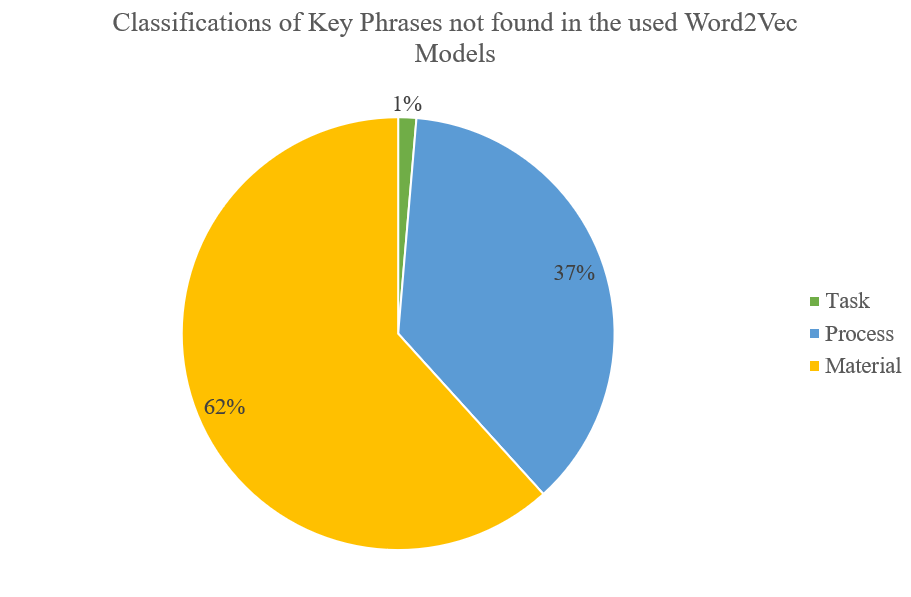
\includegraphics[width=\textwidth]{img/w2vbadtokensclasses.png}
	\caption[Key Phrase Classifications not in Word2Vec Model]{Gold standard key phrase classifications for key phrases that are not in the Word2Vec models used. 222 key phrases are included in this set.}
	\label{figure:w2vbadtokensclasses}
\end{figure}

\section{Subtask C - Relation Extraction}
\subsection{Word2Vec Usage}
Having considered Word2Vec's similarity function in the previous subtask, it shall again be utilised for this subtask - relation extraction. The goal here is to find relationships between key phrases, that can be categorised as hyponym (\textit{is-a}) and synonym (\textit{same-as}) relationships. 

To achieve this, we consider the relative distances tokens in a Word2Vec vector space hold to each other. In theory, if words A and B, of the same type of nature (for example cities), are connected in the same way (in natural language) to words C and D, of the same type of nature (for example countries), respectively, the relative distance between A and C should be very similar to that of B and D. It should also stand that the relative distance A to B is very similar to C to D. 

Therefore, the experiment here is to test if pairs of items that are synonyms share approximately the same relative distances between each other, and the same for hyponyms. The hope is to find a way to match synonym distances and hyponym distances. 

To achieve this, as usage of support vector machine was leveraged in subtask A, it shall again be used here to construct a system that can interpret the relative distance information produced by Word2Vec for given pairs of key phrases. Two proposed ideas for feature sets based off of the Word2Vec vector information, and their development, are presented below.

\subsection{SVM - Many Features}
The first attempt at constructing a SVM to interpret the meaning of Word2Vec distances shall be based on the literal vector space difference. The vector spaces in the model have dimension sizes of 300 and 1000 for Google News and Freebase respectively. As 1000 is extremely large, and Google News has a larger vocabulary than the Freebase model, this experiment will only work with the Google News Word2Vec model. Therefore each item added to the support vector machine shall have 300 features. 

The features shall be the difference between two key phrases' vectors, taken from Word2Vec. Word2Vec has a method, \texttt{.getWordVector(word)}, which returns the vector of a given word in Word2Vec space. With two vectors representing two key phrases, one vector can be subtracted from the other, and this is a data point.

Of course, as described in subtask B, Word2Vec cannot take a string of words, so instead we again tokenize the key phrase and process each token individually, summing their vectors as each is processed. Again, it is possible that some tokens in a key phrase are not significant to a phrase when trying to mathematically represent a word, so three variants on calculating the final vector of a key phrase are proposed:
\begin{itemize}
	\item Simply summing the Word2Vec vector representation of all tokens in a key phrase,
	\item Removing stop and unimportant words and summing the vectors of the remaining tokens (if the key phrase is only unimportant words as mentioned in subtask B, the algorithm reverts to summing the vectors of all the tokens anyway so the result isn't null),
	\item Using the parse information about the phrase to attempt to extract the root noun from it. Not all key phrases have nouns, and when this happens all tokens are summed together, but as the overwhelming majority of them do have a noun, selecting just this to find relations between seems sensible as this is the key part of the key phrase, and the part that would make it a synonym or hyponym.
\end{itemize}

To generate the training data, all key phrases were paired with all other key phrases (within their papers). The vector differences were all calculated, and the key phrase pairs that were hyponym or synonym relations labelled. Rather than one SVM that handled multiple labels, two SVMs were trained, one with the hyponyms labelled and the other with synonyms labelled. The thought behind this was that it would be simpler to manage training and testing as hyponyms and synonyms could be dealt with separately. As with the key phrase SVM, the RBF kernel was once again used.

Cross validation was applied to both SVMs, however, the range of values tested did not seem much change. The top row of figure \ref{figure:relsvmcv} show the cross validation results for this set of SVMs, and do not really indicate any trend. For both hyponym and synonym of extraction, \textit{C = 5} and \textit{$\gamma$ = 1} appeared to have slightly higher accuracy, but overall very little difference can be seen. The reason the accuracy is extremely high (all results are less than 0.5\% from 100\%) is because of the low amount of \textit{true case} relationship training points compared to the whole data set: 674 total relations out of 144410 possible combinations. This may prove problematic when testing on real world data, as the SVM effectively has a lack of good training data to learn off of (so may struggle to fit a good separating hyperplane).

This \textit{many features} SVM was implemented in \texttt{RelationshipSVM} (which extends from the previously described \texttt{BaseSvm}) in the Java project accompanying this report.

\begin{figure}
	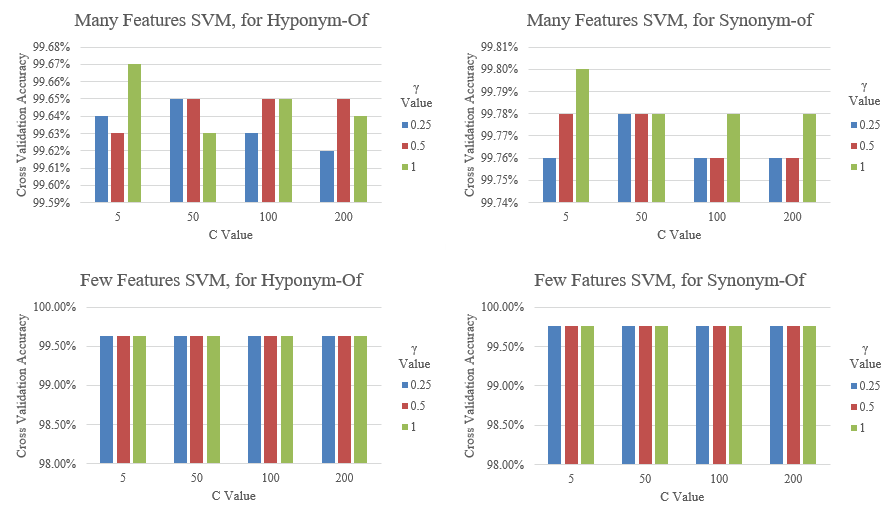
\includegraphics[width=\textwidth]{img/relsvmcrossvalidation.png}
	\caption[Relation SVM Cross Validation]{The cross validation results on both the hyponym and synonym variants of the \textit{many features} and \textit{few features} relationship SVMs.}
	\label{figure:relsvmcv}
\end{figure}

\subsection{SVM - Few Features}
Mentioned above, as the data was sparsely labelled and each point had a high feature count in the \textit{many features} SVM approach, this \textit{few features} approach aimed to reduce the complexity of the data presented in a hope it would allow for easier hyperplane fitting, meaning significantly reduced training times and hopefully a higher accuracy rate.

The idea was to reduce the vectors generated by Word2Vec to retain much of the same information in a simpler format. The result of this idea was to generate, given two key phrase vectors, the angle and the distance between the two vectors. The reason for these two metric is because these should preserve relative differences between vectors, as it is still based on the change in vector space between them.

To achieve this, the algorithm for generating a data point initially generates a vector sum of the tokens in each key phrase. With the two vectors prepared, we then calculate the following:
\begin{itemize}
	\item Euclidean distance between the two vectors:
	\begin{equation*}
	d(\overrightarrow{u}, \overrightarrow{v}) = ||\overrightarrow{u} - \overrightarrow{v}|| = \sqrt{(u_1 - v_1)^2 + (u_2 - v_2)^2 ... + (u\textsubscript{300} - v\textsubscript{300})^2}
	\end{equation*}
	\item The angle between the two vectors based on the dot product:
	\begin{equation*}
	cos(\theta) = \dfrac{\overrightarrow{u} \cdot \overrightarrow{u}}{||\overrightarrow{v}|| \cdot ||\overrightarrow{v}||}
	\end{equation*}
\end{itemize}

These two values are then used as the features of each data point. A point is generated per pair of key phrases in a document, and labelled as to whether or not they are a label. As with the \textit{many features} version, two SVMs were trained, one for hyponyms and one for synonyms. The RBF kernel was used in these SVMs.

Unfortunately, completing cross validation for this \textit{few features} SVM approach was not fruitful. The result can be seen in figure \ref{figure:relsvmcv}, with the relevant charts below that of the \textit{many features} cross validation results. Across the board for both SVMs, there is no change is accuracy with the different values tested. This likely means that no selection of relations is happening (the high accuracy is again because most of the data points should not be labelled as relationships), which does not bode well for real world tests. Given no trend has happened, it is hard to evaluate how to try to fix this issue. Theoretically, increasing the \textit{C} value may allow for the SVM to find a better hyperplane which may help, but with when \textit{C = 200}, the training time is many hours and the computer this is running on (equipped with 16 GB of memory) does not have enough memory to train further than that. Increasing \textit{C} this further simply used many gigabytes of Linux swap space on the actual disk which slows it further, and if Java is not configured to be allowed to use that much memory, it can interrupt testing as well.

This \textit{few features} SVM was implemented in \texttt{RelationshipSVM2} (which also extends from \texttt{BaseSvm}) in the Java project accompanying this report.
